\documentclass[12pt]{report}	%worth trying refman, memoir classes (memoir manual is recommended read)
\usepackage[usenames]{color}
\usepackage{titlesec}
\setcounter{secnumdepth}{2}
\setcounter{tocdepth}{2}
\usepackage[utf8]{inputenc}
\usepackage{parskip}
\usepackage{setspace}
\titleformat{\chapter}[block]
  {\normalfont\huge\bfseries}{\thechapter.}{0.5em}{\Huge}
% \titlespacing*{\chapter}{0pt}{-19pt}{0pt}
\usepackage[ampersand]{easylist}
\usepackage{graphicx}
\usepackage{svg}
\graphicspath{ {data/} }
% \usepackage{tabularx}
\usepackage{longtable}
% \usepackage{xtab}
\usepackage[breaklinks=true]{hyperref}
\hypersetup{pdfpagemode=UseOutlines}
% \usepackage{fdsymbol}
\usepackage{bm}
\usepackage[toc,page]{appendix}
% \usepackage{alltt}
% \usepackage{marvosym}
% \newcommand*{\TakeFourierOrnament}[1]{{%
% \fontencoding{U}\fontfamily{futs}\selectfont\char#1}}
% \newcommand*{\danger}{\TakeFourierOrnament{66}}
\usepackage{hyperref}
\hypersetup{
  colorlinks=true,
  linkcolor=blue!50!red,
  urlcolor=blue
}


\begin{document}
\pagenumbering{roman}
\title{Bintracker Manual}
\author{utz/irrlicht project}
\date{\today}
\maketitle
\pagenumbering{arabic}
\tableofcontents

\chapter{About}

\section{What is Bintracker?}
Bintracker is a cross-development music editor for low-level sound drivers, and a visual front-end for the \href{https://utz82.github.io/MDAL/}{Music Data Abstraction Language} (MDAL). It is designed mainly with 1-bit music engines in mind, but is by no means limited to those. Bintracker is easily extensible - additional sound drivers can be added through a plug-in system, without the need for recompiling the application itself. As long as the target platform is supported, Bintracker can handle any sound routine supported by MDAL. In the future, Bintracker will support a range of different target platforms. At the current stage however, it supports only the original Sinclair ZX Spectrum and its beeper. 

\section{License}
Bintracker and all its components are free, open source software. The bundle is released under the "Revised" (3-clause) BSD-License. This means you're basically free to use, modify, and redistribute this software both in binary as well as source form, as long as you don't pretend that I endorse what you're doing, or try to hold me responsible for any damage done. The full license terms can be found in the \texttt{docs/licenses} folder.

Bintracker includes a distribution of the \href{https://pugixml.org/}{pugixml} XML parser library, which is available under MIT license terms. See the \texttt{docs/licenses} folder for further details. Furthermore, Bintracker uses the \href{http://liballeg.org/}{Allegro5} library, which is available under the terms of the zlib License.


\chapter{Setup}
\section{General}
To make best use of Bintracker, you may want to add the following files to the \texttt{resources/roms} folder:

\texttt{zxspectrum48.rom} - The Sinclair ZX Spectrum 48K ROM.

These files are not distributed with Bintracker due to copyright restrictions.


\subsection{Windows}
No need to install anything, just unzip the bintracker package to a folder of your choice. 

\subsection{Linux/*nix}

On Linux/*nix machines, Bintracker can be build from source using either GCC or Clang. In order to do so, you will first need to install a recent version of the \href{http://liballeg.org/download.html}{Allegro5} libraries (>=5.2) as well as the according development headers. Most major distributions have Allegro5 in their repositories. On Debian, you can (su)do
\begin{verbatim}
apt-get install liballegro5-dev
\end{verbatim}
which should install Allegro5 and all necessary addons. Then simply run make to build Bintracker.


\subsection{MacOS X}
In theory, it is possible to build Bintracker on OS X, however this is untested and may require some manual tweaking. In any case, you will need \href{https://brew.sh/}{Homebrew}, standard build tools, and \href{http://liballeg.org/download.html}{Allegro5}.


\section{Customization}

You may want to set bintracker as the default application for opening .mdal files. This way, you can open your bintracker tunes by double-clicking on them.

You can also tweak a number of Bintracker's default settings by editing the \texttt{settings.ini} file. Note that the INI parser is very basic, so Bintracker may crash or simply refuse to start if certain INI settings are invalid.

The following parameters are available:

\subsubsection{XRES}
Set the horizontal resolution of the editor window in pixels. Minimum size is 720.

\subsubsection{YRES}
Set the vertical resolution of the editor window in pixels. Minimum size is 480.

\subsubsection{KBDLANG}
Set the keyboard locale. Supported locales are EN (English), FR (French), and DE (German).

\subsubsection{BGCOLOR}
Set the background colour as 24-bit RGB value (ie. standard HTML colours). Hex values must be prefixed with \$.

\subsubsection{SYSCOLOR}
Set the system colour (used for borders, scrollbars, buttons, labels etc.) as 24-bit RGB value (ie. standard HTML colours). Hex values must be prefixed with \$.

\subsubsection{ROWCOLOR}
Set the colour of data rows as 24-bit RGB value (ie. standard HTML colours). Hex values must be prefixed with \$.

\subsubsection{ROWHIGHLIGHTCOLOR}
Set the colour of highlighted data rows as 24-bit RGB value (ie. standard HTML colours). Hex values must be prefixed with \$.

\subsubsection{ROWACTIVECOLOR}
Set the colour of active data rows as 24-bit RGB value (ie. standard HTML colours). Hex values must be prefixed with \$.

\subsubsection{CURSORCOLOR}
Set the colour of the cursor as 24-bit RGB value (ie. standard HTML colours). Hex values must be prefixed with \$.

\subsubsection{SELECTIONCOLOR}
Set the colour for selections as 24-bit RGB value (ie. standard HTML colours). Hex values must be prefixed with \$.

\subsubsection{DEFAULTROWHIGHLIGHT}
Set the distance between row highlights.

\subsubsection{DEFAULTBLOCKLENGTH}
Set the standard length for new blocks.

\subsubsection{DEFAULTNUMBASE}
Set the number base. This field is currently ignored, as decimal mode is not fully implemented yet.

\subsubsection{DEFAULTCONFIG}
The default MDAL configuration to be loaded on startup.

\subsubsection{CHUNKSIZE}
The audio chunk size used by the sound emulation. A lower value means lower latency. Increase this value if you are experiencing skippy/rough audio.

\subsubsection{KEYREPEATDELAY}
The delay before key repeat is activated, as number of video frames (1/22.5 seconds).

\subsubsection{SIMPLEGFXBUFFER}
Setting this option to \texttt{false} will reduce CPU usage, but may cause flickering graphics on some platforms.


\chapter{Introduction}
\section{General Concepts}

Bintracker belongs to a class of music editors known as \href{https://en.wikipedia.org/wiki/Tracker_\%28music_software\%29}{trackers}. Characteristic traits of trackers include:

\begin{itemize}
\item a minimalistic, number based interface
\item keyboard-centric workflow
\item vertical representation of time flow
\end{itemize}

In case you are completely new to using trackers, you may want to first familiarize yourself with the jacks of the trade by reading the \href{http://resources.openmpt.org/tracker_handbook/handbook.htm}{The Tracker's Handbook} before continuing with this manual.

Quite likely you already know what a tracker is. In this case, you will find that Bintracker is not much different from other trackers you may have used. However, Bintracker does have a few quirks - read up on those in the next section.



\section{Differences with other Trackers}

As Bintracker is primarily a front-end for the MDAL markup language, there are some notable differences with other trackers such as Famitracker, Deflemask, or OpenMPT.

Most existing trackers differentiate between \textit{patterns}, \textit{instruments}, and possibly various types of \textit{ornaments} or \textit{effect tables}. Bintracker however does not make these distinctions. In MDAL, and consequently in Bintracker, everything is a \textit{block}. Patterns are blocks. Effect tables are blocks. Volume envelopes are blocks. Samples are blocks. 

In practise though, this will have little to no impact on your workflow. Pattern blocks still act like traditional patterns, and you'll link them together in a traditional sequence. Effect table blocks will act like effect tables, envelope blocks will act like envelopes, and sample blocks will act like samples.

The reason for doing away with these traditional distinctions is that the sound engines supported by MDAL widely differ in their capabilities. Some engines only support plain patterns, without extraneous tables or instruments. Others may make extensive use of tick-based envelopes or samples. Ultimately, which types of blocks are available depends entirely on the engine you use.

Another common concept of other trackers that does not exist in Bintracker is the notion of \textit{tracks}, also known as \textit{channels}. A channel, as presented in "normal" trackers, will almost always consist of a note column, followed by various columns for instrument, volume, and effect settings. Often, these channels correspond to the hardware channels available on the tracker's target sound chip. 

Since bintracker is mainly dealing with 1-bit sound-routines, this concept makes not a lot of sense here. In a 1-bit engine, several tone channels may share a common effect setting, or may impact each other in some way. In fact, the number of available tone channels itself may be flexible, and subject to change depending on the effect settings.

Hence, bintracker uses independent \textit{columns}. Each column corresponds to a \textit{command}. There are different flavours of commands, such as \textit{note commands}, \textit{parameters} for specifying various sound settings, and \textit{references} to other blocks, linking instruments, samples, or effect tables. In addition to the column commands, there may also be commands available that are not tied to a column. Such commands may for example be used to specify a tune's author and title, or a global speed setting. Again, which channels are available as well as their function depends on the engine in use.



\chapter{Keyboard Shortcuts}
\section{General Keys}

\begin{longtable}{p{0.33\textwidth} p{0.60\textwidth} }
\textbf{key} & \textbf{function} \\
\hline
\\
\textbf{F2} & Show engine info \\
\\
\textbf{F5} & Play from start \\
\textbf{F6} & Play from current position \\
\textbf{F7} & Play pattern \\
\textbf{F8} & Stop \\
\\
\textbf{Tab} & Toggle block/list \\
\textbf{Ctrl\(\bm{+}\)Tab} & Cycle through block tabs \\
\\
\textbf{Esc} & Abort action \\
\\
\textbf{Ctrl\(\bm{+}\)Z} & Undo \\
\textbf{Ctrl\(\bm{+}\)Y} & Redo \\
\\
\textbf{Ctrl\(\bm{+}\)O} & Open File... \\
\textbf{Ctrl\(\bm{+}\)S} & Save File \\
\textbf{Ctrl\(\bm{+}\)Shift\(\bm{+}\)S} & Save File As... \\
\\
\textbf{Alt\(\bm{+}\)1..6} & set base octave to 1..6 \\
\textbf{Alt\(\bm{+}\)7/8} & decrement/increment base octave \\
\textbf{Alt\(\bm{+}\)Page Up/Down} & increment/decrement edit step (auto-inc) \\
\\
\end{longtable}


\section{General Tab Keys}

\begin{longtable}{p{0.33\textwidth} p{0.60\textwidth} }
\textbf{key} & \textbf{function} \\
\hline
\\
\textbf{Up/Down} & Move cursor up/down \\
\textbf{a-z, 0-9, Space} & enter data (context sensitive) \\
\textbf{Enter} & complete text input \\
\textbf{Backspace} & delete last char (text input only) \\
\\
\end{longtable}



\section{Block Keys}
\begin{longtable}{p{0.33\textwidth} p{0.60\textwidth} }
\textbf{key} & \textbf{function} \\
\hline
\\
\textit{\textbf{arrow keys}} & Move cursor \\
\textbf{Page Up/Down} & Move cursor up/down 16 rows\\
\textbf{Home/End} & Move cursor to first/last row\\
\textbf{Alt\(\bm{+}\)left/right} & show previous/next block \\
\textbf{Enter} & reference columns: show block at cursor \\
 & text commands: complete input \\
\textbf{Backspace} & text columns: delete last char \\
\\
\textbf{a-z, 0-9} & enter notes/data (context sensitive) \\
\textbf{1} & note colums: rest note (if available) \\
\textbf{k} & note colums: noise note (if available) \\
\textbf{Space} & clear field \\
\textbf{\(\bm{+-*/}\)\&$\vert$\textasciicircum} & set modifier (if available) \\
\textbf{\(\bm{=}\)} & remove modifier (if available) \\
\textbf{.} & repeat previous value \\
\\
\textbf{Ins} & insert field \\
\textbf{Del} & delete (cut) field \\
\textbf{Alt\(\bm{+}\)V, Alt\(\bm{+}\)Ins} & Insert row \\
\textbf{Alt\(\bm{+}\)Del} & Delete (cut) row \\
\textbf{Alt\(\bm{+}\)\(\bm{+}\)} & Add row (increment block length) \\
\textbf{Alt\(\bm{+}\)\(\bm{-}\)} & Remove row (decrement block length) \\
\\
\textbf{Alt\(\bm{+}\)R} & Rename block \\
\textbf{Alt\(\bm{+}\)X} & Expand block \\
\textbf{Alt\(\bm{+}\)Shift\(\bm{+}\)X} & Shrink block \\
\\
\textbf{Ctrl\(\bm{+}\)A} & Select all \\
\textbf{Shift\(\bm{+}\)\textit{arrow keys}} &\\
\textbf{Shift\(\bm{+}\)Page Up/Down} & Select fields\\
\textbf{Shift\(\bm{+}\)Home/End} & \\
\\
\textbf{Ctrl\(\bm{+}\)C} & Copy selection to clipboard \\
\textbf{Ctrl\(\bm{+}\)X} & Cut selection \\
\textbf{Ctrl\(\bm{+}\)Del} & Delete selection (cut and shift) \\
\textbf{Ctrl\(\bm{+}\)V} & Paste from clipboard (overwrite) \\
\textbf{Ctrl\(\bm{+}\)Shift\(\bm{+}\)V} & Porous paste \\
\textbf{Ctrl\(\bm{+}\)Alt\(\bm{+}\)V} & Inverse porous paste \\
\textbf{Ctrl\(\bm{+}\)P} & Insert (paste and shift) \\
\\
\textbf{Ctrl\(\bm{+}\)F} & Fill selection/cursor-end from clipboard \\
\textbf{Ctrl\(\bm{+}\)Shift\(\bm{+}\)F} & Porous fill \\
\\
\textbf{Ctrl\(\bm{+}\)I} & Interpolate selection (linear) \\
\textbf{Ctrl\(\bm{+}\)Shift\(\bm{+}\)I} & Interpolate selection (reciprocal) \\
\textbf{Ctrl\(\bm{+}\)Alt\(\bm{+}\)I} & Interpolate selection (cubic) \\
\\
\textbf{Ctrl\(\bm{+}\)R} & Reverse selection \\
\\
\textbf{Ctrl\(\bm{+}\)U} & Transpose selection 1 semitone up \\
\textbf{Ctrl\(\bm{+}\)Shift\(\bm{+}\)U} & Transpose 1 octave up \\
\textbf{Ctrl\(\bm{+}\)D} & Transpose 1 semitone down \\
\textbf{Ctrl\(\bm{+}\)Shift\(\bm{+}\)D} & Transpose 1 octave down \\
\\
\end{longtable}


\section{Sequence/Block List Keys}

\begin{longtable}{p{0.33\textwidth} p{0.60\textwidth} }
\textbf{key} & \textbf{function} \\
\hline
\\
\textbf{Up/Down} & Move cursor up/down\\
\\
\textbf{Alt\(\bm{+}\)\(\bm{+}\)} & Add new block/step \\
\textbf{Del} & Delete step/block \\
\textbf{Alt\(\bm{+}\)C} & Clone block/step \\
\\
\textit{\textbf{Sequence only}} & \\
\hline
\\
\textbf{PgUp/PgDn} & Move cursor up/down 16 rows \\
\textbf{Home/End} & Move cursor to start/end \\
\\
\textbf{Ins, Alt\(\bm{+}\)V} & Insert step \\
\\
\textbf{Ctrl\(\bm{+}\)A} & Select all \\
\textbf{Shift\(\bm{+}\)\textit{up/down}} &\\
\textbf{Shift\(\bm{+}\)Page Up/Down} & Select steps\\
\textbf{Shift\(\bm{+}\)Home/End} & \\
\\
\textbf{Ctrl\(\bm{+}\)C} & Copy selection to clipboard \\
\textbf{Ctrl\(\bm{+}\)Del} & Delete selection (cut and shift) \\
\textbf{Ctrl\(\bm{+}\)V} & Paste from clipboard (overwrite) \\
\textbf{Ctrl\(\bm{+}\)P} & Insert (paste and shift) \\
\end{longtable}


\chapter{Using Bintracker}
\section{The Main Menu}

The main menu is where you will find... all the important stuff, of course.


\begin{itemize}
\item \textbf{File}
\begin{itemize}
\item \textbf{New...} - Loads a new blank MDAL module file for a sound engine of your choice.
\item \textbf{Open...} - Opens an existing MDAL module file.
\item \textbf{Save} - Saves the current MDAL module file. Any unused blocks will not be saved.
\item \textbf{Save As...} - Saves a copy of the current MDAL module file with a new name.
\item \textbf{Export...} - Export the current MDAL module to a range of different formats. Available export formats depend on the module's target platform.
\item \textbf{Exit} - Quits Bintracker. Unused blocks are permanently lost.
\end{itemize}
\item \textbf{Edit}
\begin{itemize}
\item \textbf{Undo} - Reverts the last edit action. Undo is limited to around 100 steps.
\item \textbf{Redo} - Reverts the last undo action.
\item \textbf{Select All} - Select the entire block or pattern sequence, depending on the cursor position.
\item \textbf{Copy} - Copies the current selection.
\item \textbf{Cut} - Cuts the current selection. Cutting will not shift the data following the selection.
\item \textbf{Delete} - Cut the current selection, and shift up the following data.
\item \textbf{Insert} - Insert the copied/cut/deleted selection from the clipboard at the current cursor position, shifting the following data.
\item \textbf{Paste} - Paste the copied/cut/deleted selection from the clipboard at the current cursor position, overwriting the following data.
\item \textbf{Porous Paste} - Merge the copied/cut/deleted selection from the clipboard into the data following at the current cursor position, keeping the \textit{current} data intact.
\item \textbf{Inverse Porous Paste} - Merge the copied/cut/deleted selection from the clipboard into the data following at the current cursor position, keeping the \textit{copied} data intact.
\item \textbf{Interpolate...}
\begin{itemize}
\item \textbf{Linear} - Interpolate the selected data, using a linear function.
\item \textbf{Cubic} - Interpolate the selected data, using a cubic function.
\item \textbf{Reciprocal} - Interpolate the selected data, using a reciprocal function.
\end{itemize}
\item \textbf{Fill...}
\begin{itemize}
\item \textbf{Overwrite} - Fill the current selection with data from the clipboard. If no selection is made, fill the current column, starting at the current cursor position.
\item \textbf{Porous} - Fill gaps in the currently selected data with data from the clipboard. If no selection is made, fill gaps in the current column data, starting at the current cursor position.
\end{itemize}
\item \textbf{Transpose...}
\begin{itemize}
\item \textbf{+1 semitone} - Transpose the currently selected note data one semitone upwards.
\item \textbf{-1 semitone} - Transpose the currently selected note data one semitone downwards.
\item \textbf{+1 octave} - Transpose the currently selected note data one octave upwards.
\item \textbf{+1 octave} - Transpose the currently selected note data one octave upwards.
\end{itemize}
\item \textbf{Reverse} - Reverse the current selection.
\item \textbf{Randomize} - Fill the selection with random data.
\end{itemize}
\item \textbf{Play}
\begin{itemize}
\item \textbf{Play from Start} - Play back the current module from the beginning.
\item \textbf{Play from Current Position} - Play back the current module from the current cursor position.
\item \textbf{Play Pattern} - Play and loop the current pattern.
\item \textbf{Stop} - Stop playback.
\end{itemize}
\item \textbf{Help}
\begin{itemize}
\item \textbf{About} - Show a little box with version info and some other stuff.
\end{itemize}
\end{itemize}

\section{Main Interface Overview}

{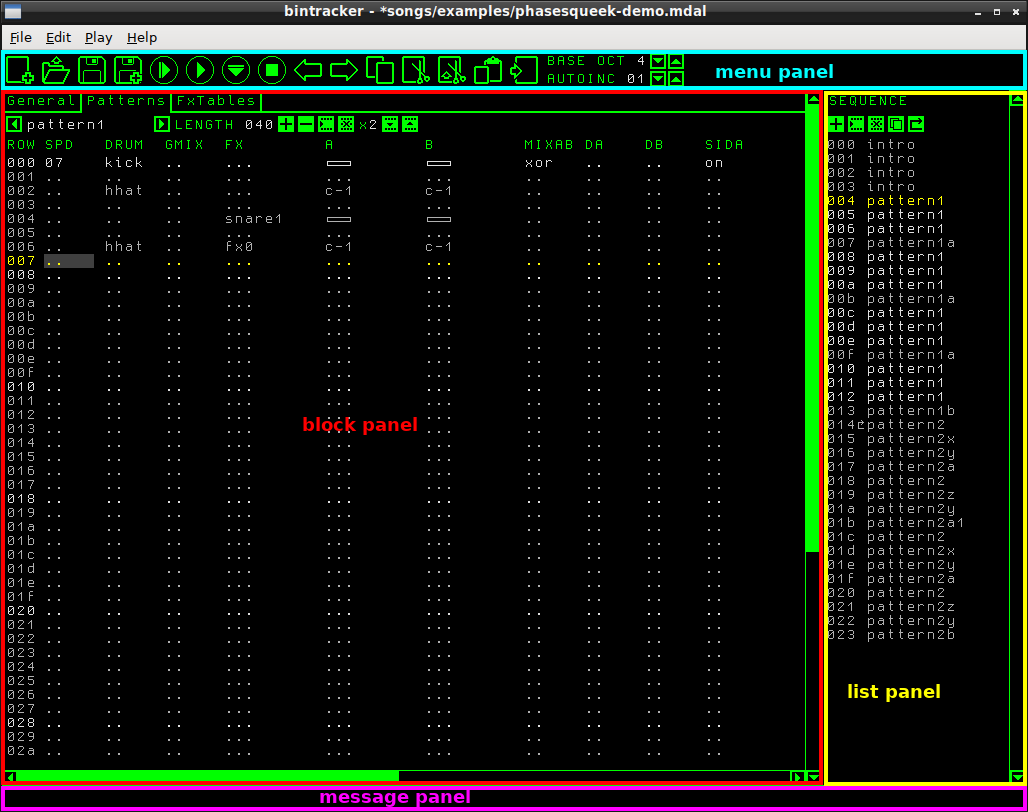
\includegraphics[width=\textwidth]{overview}}

\subsection{The Menu Panel}

The menu panel, located at the top of the editor window, replicates some of the functions of the main menu for easy access with a single mouse click. The following functions are available:

\begin{tabular}{llll}
\raisebox{-.3\height}{
\includegraphics[width=28pt]{new_file}} & Create New File & \raisebox{-.3\height}{
\includegraphics[width=28pt]{open}} & Open File \\
\rule{0pt}{2em}\raisebox{-.3\height}{
\includegraphics[width=28pt]{save}} & Save File & \raisebox{-.3\height}{
\includegraphics[width=28pt]{save_as}} & Save File As... \\
\rule{0pt}{2em}\raisebox{-.3\height}{
\includegraphics[width=28pt]{play_from_start}} & Play from Start & \raisebox{-.3\height}{
\includegraphics[width=28pt]{play}} & Play from Current Position \\
\end{tabular}

\begin{tabular}{llll}
\raisebox{-.3\height}{
\includegraphics[width=28pt]{play_pattern}} & Play Pattern & \raisebox{-.3\height}{
\includegraphics[width=28pt]{stop}} & Stop \\
\rule{0pt}{2em}\raisebox{-.3\height}{
\includegraphics[width=28pt]{undo}} & Undo & \raisebox{-.3\height}{
\includegraphics[width=28pt]{redo}} & Redo \\
\rule{0pt}{2em}\raisebox{-.3\height}{
\includegraphics[width=28pt]{copy}} & Copy & \raisebox{-.3\height}{
\includegraphics[width=28pt]{cut}} & Cut... \\
\rule{0pt}{2em}\raisebox{-.3\height}{
\includegraphics[width=28pt]{cut_and_move_up}} & Delete (Cut and Shift) & \raisebox{-.3\height}{
\includegraphics[width=28pt]{paste_over}} & Paste \\
\rule{0pt}{2em}\raisebox{-.3\height}{
\includegraphics[width=28pt]{insert}} & Insert (Paste and Shift) & & \\
\end{tabular}

Furthermore, the menu panel displays the current base octave (BASE OCT) and auto-increment step (AUTOINC) settings. You can change these settings with the arrow buttons next to them. You can also set the base octave directly by pressing \textbf{Alt\(\bm{+}\)0..6}, or decrement/increment it with \textbf{Alt\(\bm{+}\)7/8}. The auto-increment step can be decremented/incremented by pressing \textbf{Alt\(\bm{+}\) PageUp/PageDown}.

\subsection{The Block Panel}

The block panel occupies the main portion of the editor window. It consists of two or more tabs, depending on the sound engine used. The General tab is used to display and edit the tune's global settings and commands. The remaining tabs are used to edit the tune's patterns and other data blocks, if any are used by the engine's configuration. Information on using the block panel can be found in the sections on \nameref{subsec:editing-globals}, \nameref{subsec:editing-patterns}, and \nameref{subsec:editing-blocks}.

\subsection{The List Panel}

The list panel, located to the right of the block panel, is used in different ways, depending on the active tab of the block panel. When the General tab is active, the list tab will show various bits of information about the current tune. When the Patterns tab is active, the list panel will display the song sequence. When any other tab is active, the list panel will show corresponding list of blocks. Information on using the list panel can be found in the sections on \nameref{subsec:editing-sequence} and \nameref{subsec:editing-block-list}.

\subsection{The Message Panel}


The message panel, located at the bottom of the editor window, is used to display tooltips and hints about keyboard shortcuts, as well as error messages.

\section{Composing Music: A Walk-Through}

The following sections give a brief overview over the Bintracker work flow. After reading these, you should have enough knowledge to get started with composing your own tunes in Bintracker.

\subsection{Choosing a Sound Engine}

Bintracker supports multiple sound engines, and what you see on screen can vary considerably depending on which sound engine you chose. For the purpose of this walk-through, we are going to use the PhaseSqueek engine. (Note that documentation on the various engines supported by Bintracker is not part of this manual. Engine documentation can be found in the \texttt{docs/engines} folder, or by pressing \textbf{F2}.)

To get started, launch the Bintracker program. Then, click on the \textit{File} menu item and select \textit{New... $\rightarrow$ PhaseSqueek}. This will create a new, empty PhaseSqueek module.

\subsection{Editing Global Song Settings}
\label{subsec:editing-globals}

Before we dive into the really heavy stuff, let's edit some global settings of our tune. Activate the \textbf{General tab} by clicking on \textit{General} just below the menu panel, near the left edge. A list with three MDAL commands (AUTHOR, TITLE, and GSPD) with editable fields next to them will appear. Use the arrow up and arrow down keys to move the cursor, or simply click on the field you wish to edit. To edit a field, simply start typing on your keyboard. 

The AUTHOR and TITLE commands set the song author and title, respectively. Note that only lowercase letters are allowed at the moment. Any invalid characters will be rejected. To complete your input, hit \textbf{Enter}. To cancel your input, hit \textbf{Esc}.

The GSPD command sets the global song speed. Note that by default, Bintracker uses hexadecimal numbers, so possible values for this field range from 00 to FF (255 in decimal). A higher value means lower speed. Currently, GSPD is set to 10 (16 in hexadecimal). That's quite slow, so let's set it to 08 by moving the cursor to the GSPD field, then typing 08. Simple, right? Ok, let's move on to the pattern editor.

\subsection{Editing Patterns}
\label{subsec:editing-patterns}

Patterns are the main building blocks of your tune. This is where you construct your actual melodies and rhythms. The sheet music equivalent of a pattern would be a phrase, except that patterns are usually longer than phrases.

To open the pattern editor, click on the \textbf{Patterns tab} at the top of the block panel, next to the General tab. A classic, good ol' pattern view will appear.

At the top left corner of the block tab, the name of the pattern is shown, sandwiched between two arrow buttons (these can be used to cycle through patterns once you have a few more of them). Right now the current pattern is called "pattern00". Click on the name to change it - let's call it "intro" for now. Once you hit enter, the cursor will automatically return to the main pattern data block.

On the left side, below the ROW label, the row numbers of the pattern are shown. Next to the row label, you will find all the available MDAL pattern commands, each with a column of editable fields below. There are a few different types of MDAL commands, and the editor will act differently depending on the command type. We will cover all the common types in this tutorial. In fact, we've already covered \textit{text commands} (AUTHOR, TITLE) and plain \textit{data commands} (GSPD) in the previous section. To find out what each command does on a given engine, press \textbf{F2}.

The first command is SPD. This sets the speed for the current row, and the ones that follow after it, until the command is set again. If you do not set this command, the value from the GSPD command on the General tab will be used. We've already set GSPD to a reasonable value, so there's no need to set the SPD command right now. If you did enter some value by accident, you can simply clear it by pressing \textbf{Space}.

Move the cursor to the next column (labelled DRUM), either with the arrow keys or by clicking on the desired field. The DRUM command triggers a click drum. This command type uses an MDAL feature called \textit{substitution}, which means you don't enter numbers here, but rather chose from a list of keywords. Type any letter or number on your keyboard, and a list of available keywords will be displayed below the field you are editing. In our case, the list contains two items, \textit{kick} and \textit{hhat}. Start typing the name of the keyword you want to use, eg. type \textbf{k} for a kick drum, or \textbf{h} for a hi-hat. As there are only two items, typing k or h will complete the input. However, some commands use more keywords, so you might need to type a few more characters before the choice becomes conclusive. Note that if we would have pressed k or h at the beginning, the field would have been set instantly, without displaying the options list. You can also select keywords with the arrow keys, and confirm the choice with \textbf{Enter}.

The next column is labelled GMIX. GMIX sets the general channel mixing algorithm. It's another substitution command. We'll leave it alone for now.

The following column, labelled FX, sets the fx table to be used. It is a so-called \textit{reference command}, which means it refers to another block type, in this case an FxTable. Reference commands work similar to substitution commands, that means when you start typing, you will be displayed a list of options. We haven't created any fx tables yet, so let's skip this command for now.

The following column, labelled "A", sets the note for the first oscillator (in other words, A is a \textit{note command}). On note commands, your keyboard acts like a piano keyboard. Key \textbf{Y} corresponds to note \textit{C}, \textbf{S} corresponds to \textit{C\#}, \textbf{X} corresponds to \textit{D}, and so forth. This is repeated in the upper half of the keyboard, eg. \textbf{Q} is \textit{C} one octave up, \textbf{2} is \textit{C\#}, and so forth. To put in a rest, press key \textbf{1}. The base octave can be set in the menu panel, by clicking the arrows next to the BASE OCT field. You can also set the base octave directly by pressing \textbf{Alt\(\bm{+}\)0..6}, or decrement/increment it with \textbf{Alt\(\bm{+}\)7/8}. Note that some engines may limit the range of available notes.

Feel free to enter a few notes before moving on to the next column, labelled "B". As you might have guessed, B sets the note for the second oscillator. Now, a special feature of the PhaseSqueek engine is that by default, it combines two oscillators into one channel. That means A and B are not independent from each other, but rather form one combined sound. 

In effect, this also means that we probably don't want to enter arbitrary notes into column B. Rather, a smart move would be to duplicate the notes in colum A, but with a little bit of detune. Here's how to do that. First, move the cursor back to column A. Now, hold down the \textbf{Shift} key and select the notes you entered with the \textbf{arrow up/down} keys. When you're done, press \textbf{Ctrl\(\bm{+}\)C} to copy the selection. Now move the cursor to column B and press \textbf{Ctrl\(\bm{+}\)V} to paste the current selection. Column A and B should now contain the same data. If you've accidentally pasted at the wrong position, you can move things down or up by pressing \textbf{Ins} or \textbf{Del}. 

If all is good, it's time to work on that detune. Move the cursor to the first note in column B, and press \textbf{\(\bm{+}\)}, followed by \textbf{1}, followed by \textbf{Enter}. The field will now display \textless\textit{notename}\textgreater+0001. Congratulations, you've just used a \textit{modifier} for the first time. Repeat this for the other notes you may have pasted into column B. 

Note that not all engines support modifiers. Also, \textbf{while Bintracker normally checks the validity of your input, this is not the case with modifiers}. It is entirely possible to crash an engine by feeding it invalid data through modifiers.

Now it's time to check the result. Press \textbf{F7} to play the pattern, or click the corresponding button in the menu panel. Pressing \textbf{F8} stops playback. You can continue editing while the player is running. However, the player is not updated instantly. Rather, it will fetch new data once it has played the entire pattern and loops back to the beginning.

The other pattern commands work in the same way as the ones we have already covered. MIXAB sets the mixing algorithm (using substitution), DA and DB change the duty cycle setting for osciallators A and B (plain 8-bit data command like GSPD/SPD), SIDA and SIDB enable or disable the SID duty sweep effect for osc A/B (substitution), ESA and ESB set the Earth Shaker effect modifier for osc A/B (plain 8-bit data), and PAB sets the phase offset between the two oscillators (16-bit plain data). The whole set is then repeated for osciallators C and D, except that the ESx commands are replaced with command NC, which enables or disables Noise mode for oscillator C. Note that for noise mode, you should use a special note (frequency divider) on column C. This "noise" note is located on key \textbf{k}.

This covers most of the command types available in MDAL/Bintracker. One additional command type not covered here will be explained in the section on \nameref{subsec:editing-blocks}.

\subsection{Sequence Editing}
\label{subsec:editing-sequence}

The sequence allows you to combine multiple patterns into a song, by specifying the order in which the patterns should be played.

When the Patterns tab is active in the block panel, the sequence will be displayed in the list panel. You can toggle between the block panel and the list panel by pressing the \textbf{Tab} key, or simply click on the panel you want to use.

When looking at the sequence, you will realize that it currently only holds a single line, which reads 000@pattern00. \textit{000} is the step number, or order position, if you will. The @ is actually a small right-pointing arrow with an L attached. It specifies the loop point, that is the point in the sequence that the player will jump to once it has finished playing the tune. \textit{pattern00} is the pattern that currently selected for this sequence step.

Let's duplicate pattern00. We can do so by selecting sequence step 000 with the cursor and pressing \textbf{Ins}, or by clicking the Insert button ({
\includegraphics[width=10pt]{button_insert}}). Now move the cursor down to step 001, and press \textbf{Alt\(\bm{+}\)C}, or click the Clone button ({
\includegraphics[width=10pt]{button_clone}}). This creates a copy of the pattern on the current step. The new pattern will receive some generic name (like "blk0"), which you can change later on the block panel. If you wish, you can now change some things in the new pattern.

You may have noticed that by inserting a new sequence step, the sequence loop point got shifted down to step 001. This is because inserting always happens on the current cursor position (so in fact the new step got inserted at position 000, and the old step moved down to step 001). To move the loop point to another step, move the cursor to that step and press \textbf{Alt\(\bm{+}\)L}, or click the loop point button ({
\includegraphics[width=10pt]{button_looppoint}}).

Instead of cloning an existing pattern, you can also create an entirely new one by pressing \textbf{Alt\(\bm{+}\)\(\bm{+}\)}, or by clicking the Add Step button ({
\includegraphics[width=10pt]{button_plus}}). The new pattern will be appended at the end of the sequence. To insert the pattern at another sequence step, move to that step and type the first letter of the pattern's name. If your choice was unambiguous, the sequence step will be set to the new pattern. Otherwise, a list of options will appear, and you keep typing until only one option is left. Alternatively, you can select an option with the arrow keys, and confirm the choice with \textbf{Enter}.(To cancel this process, press \textbf{Esc}).

You can delete sequence steps by pressing \textbf{Del}, or by clicking the Delete Step button ({
\includegraphics[width=10pt]{button_remove}}). Removed patterns will not be deleted immediately, but will be lost eventually if they are not used at any other sequence step (see below).

Aside from inserting and creating new steps, you can also copy/paste/insert multiple steps, much like in the pattern editor.

\textbf{Important: Any patterns not used in the sequence will not be saved in your module file, and will be lost when you exit Bintracker or load another track.}


\subsection{Editing Non-Pattern Blocks}
\label{subsec:editing-blocks}

Editing non-pattern blocks works exactly like editing patterns, except that any notes will not be played when you enter them.

PhaseSqueek uses one non-pattern block type called FxTables. In the pattern editor, you can select which FxTable to use at a given point with the FX command.

Clicking on the "FxTable" tab in the block panel will show the only instance of this block type that we have right now. It's called "fx0", and it consists of only a single row. This is the default block, used if you don't specify any parameter for the FX pattern command. You probably want to leave it alone, and instead create a new block (see the following section on how to create a new FxTable block).

PhaseSqueek's FxTables use mostly the same commands as the patterns. However, there are two commands that are not available for patterns: STOP and JUMP. The engine info (press \textbf{F2} to view it) will tell us that one of these commands must be used at the end of each FxTable block. JUMP is a regular reference command, much like the FX pattern command. STOP, on the other hand, is a special command type we have not encountered yet: The \textit{auto command}. Auto commands do not take any arguments/parameters, they can only be \textit{set}. Pressing any alphanumeric key will set an auto command, indicated by the word "set" in the command field. Pressing \textbf{Space} clears an auto command field, like any other command type.


\subsection{Editing A Block List}
\label{subsec:editing-block-list}

When editing a non-pattern block, a list of blocks of that type will appear in the list panel. Editing this block list is somewhat different from editing the sequence. The main difference is that there are no steps to edit here, of course. Consequently, you cannot insert items at arbitrary positions. There is no copy/paste available either. You can only add new blocks (by pressing \textbf{Alt\(\bm{+}\)\(\bm{+}\)}, or by clicking the Add Block button {
\includegraphics[width=10pt]{button_plus}}), clone them (\textbf{Alt\(\bm{+}\)C} or {
\includegraphics[width=10pt]{button_clone}}), or delete them (\textbf{Alt\(\bm{+}\)Delete} or ({
\includegraphics[width=10pt]{button_remove}}). Unlike deleting a sequence step, deleting a block from the block list will immediately delete it.


\chapter{Adding New Engines}

You can add support for your own sound engines to Bintracker, provided the target machine is supported. At the moment, only the ZX Spectrum 48K is supported.
{\sloppy
In order to add an engine to Bintracker, you will need to write an MDAL configuration file. For information on how to write MDAL configurations, refer to the \href{https://github.com/utz82/MDAL/wiki}{MDAL wiki}. The .mdal file must be placed in the \texttt{engines/config} folder. Additionally, you must register the configuration in \texttt{engines/config/configlist}.
}
Furthermore, you must create a subfolder in \texttt{engines} folder, with the exact same name as your MDAL configuration file (without the .mdal extension). This folder must contain the following:

\begin{itemize}
\item The assembly source code of your engine. It must be named \texttt{main.asm}, and must be self-contained (eg. must not include any other files, and must include all the necessary definitions, equates, etc.).
\item A compiled binary of your engine (without any music data) that loops when the end of the sequence is reached. It must be named \texttt{main.bin}.
\item A compiled binary of your engine (without any music data) that exits when the end of the sequence is reached. It must be named \allowbreak\texttt{main\_no\_loop.bin}.
\item An \texttt{equates.h} header containing at least the following equates:
\begin{itemize}
\item \texttt{breakpoint\_init} - The start adress of your compiled engine.
\item \texttt{breakpoint\_exit} - The exit point of your compiled non-looping version of the engine.
\item \texttt{breakpoint\_reload} - The adress executed immediately before looping the sequence in the looping version of the engine.
\item \texttt{loop\_point\_patch} - The adress of the hard-coded pointer that is loaded on looping the sequence, if your engine uses such a construct.
\item \texttt{rest} - The value of rests, if supported by your engine.
\item \texttt{noise} - The seed for noise generation, if supported by your engine.
\item Names for all the notes supported by your engine, and their respective frequency dividers or table lookup values. Note names must be given in lower-case letters. Sharp notes are denoted by appending \textit{-is} to the note name (German notation). Bintracker does not support flats.
\end{itemize}
Equates must be specified with \texttt{equ}, hexadecimal numbers must be prefixed with \$.
\end{itemize}


\chapter{Thanks and Greetings}

Massive thanks and warm-hearted greetings go out to:

\textbf{linda8bit} for moral, emotional, and financial support

\textbf{Shiru} for his 1-bit engines, 1tracker, and his invaluable advice on asm and beeper matters

\textbf{Chris Cowley} for Beepola, and for showing the middle finger to the WOS clan

\textbf{AtariTufty} and \textbf{Garvalf} for testing and feedback, and for keeping the 1-bit scene alive

\textbf{Alone Coder} and {introspec} for all the coding tricks

\textbf{Simon Jonassen} for forcing me on a trip to 6809 land every once in a while

\textbf{Mister Beep} for turning me into a 1-bit addict

\textbf{puke7} for BattleOfTheBits.org

and last but not least, everybody still hacking away and creating art on home computers and other obsolete hardware!


\end{document}